\chapter{Livello Applicativo}
Il \emph{livello Applicativo} è l’ultimo livello dello \emph{stack protocollare TCP/IP}
e costituisce un’interfaccia per i processi che intendono comunicare sulla rete.

Vediamo più nel dettaglio le caratteristiche e le funzionalità, o meglio i
\emph{protocolli}, forniti da questo livello.

\section{Applicazioni di rete}
Uno degli utilizzi più diffusi della rete è la creazione di \emph{applicazioni di
rete}, ovvero applicazioni software diffuse su più calcolatori.

\subsection{Architetture di applicazioni di rete}
Le \emph{applicazioni di rete} possono essere basate su architetture diverse:
\begin{itemize}
    \item \emph{Client-server}: esistono \emph{server} che offrono servizi ad
    altri \emph{host} detti \emph{client}. I \emph{client} possono
    comunicare soltanto con i \emph{server};
    \item \emph{\gls{glos:P2P}}: non esistono \emph{server}, ma tutti gli
    \emph{host} sono pari tra loro. Ciascun \emph{host}, o \emph{peer}, può
    comunicare con qualsiasi altro \emph{peer};
    \item \emph{Architetture ibride}: sono architetture che hanno sia componenti
    \emph{client-server} che \emph{peer-to-peer};
    \item \emph{Cloud computing}: le risorse sono distribuite su uno o più server
    dislocati nel territorio e sono virtualizzate in modo che ogni utente
    possa utilizzare solo le risorse di cui ha bisogno;
\end{itemize}
Ma vediamole più nel dettaglio.

\paragraph{Architettura client-server}
Nelle reti basate sul modello \emph{Client-Server}, esiste un \emph{server}
centrale al quale molti \emph{client} si connettono per richiedere una risorsa o
usufruire di un servizio. Il \emph{server} deve essere sempre attivo e avere un
\emph{indirizzo IP} fisso, così da essere raggiungibile dai \emph{client}, i
quali, possono comunicare solo con lui e non tra loro.

\bigskip\noindent
Esistono quindi 2 entità:
\begin{itemize}
    \item \emph{Client}: si tratta di un componente hardware o software che invia
    delle richieste al \emph{server} e attende che questo risponda per poterne
    elaborare la risposta;
    \item \emph{Server}: si occupa di soddisfare le richieste ricevute dai
    \emph{client} e di restituire loro il risultato delle suddette richieste;
\end{itemize}
Tale modello ha come principale vantaggio la semplicità di gestione delle risorse
condivise, che risiedono tutte nel \emph{server}. Inoltre, permette di ridurre i
costi lato \emph{client} perché non è necessario che questi abbiano prestazioni
elevate. Tuttavia, nel caso di guasti o malfunzionamenti del \emph{server},
l’intera rete potrebbe risultare rallentata o inutilizzabile.

\begin{figure}[h]
    \centering
    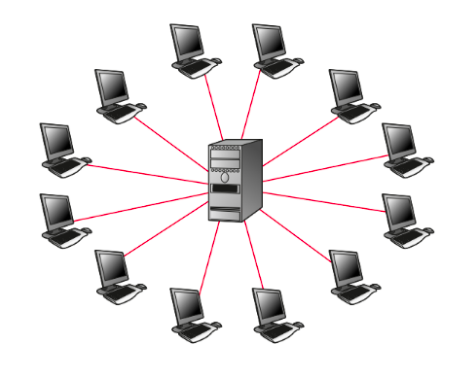
\includegraphics[width=0.4\textwidth]{modello-client-server.png}
    \caption{Schema architettura \emph{client-server}}
\end{figure}

\paragraph{Architettura P2P}
Il modello \emph{P2P} prevede la presenza di entità autonome dette \emph{peer}
che scambiano tra di loro delle risorse. Ogni \emph{peer} può sia condividere
risorse che richiederne.

Esistono diversi tipi di architetture \emph{P2P}:
\begin{itemize}
    \item \emph{P2P decentralizzato}: ogni \emph{peer} svolge sia la funzione di
    server che di client. Il sistema è in grado di adattarsi autonomamente a un
    cambiamento nei nodi partecipanti senza richiedere interventi esterni e
    mantenendo attiva la rete;
    \item \emph{P2P centralizzato}: Esiste un server centrale detto
    \emph{directory server} che contiene informazioni utili alla localizzazione
    delle risorse tra i \emph{peer}. Ogni \emph{peer} informa il server del
    tipo di risorse che intende condividere, mentre, quando ne richiede una,
    chiede al \emph{directory server} di localizzarla;
    \item \emph{P2P ibrido}: Esistono alcuni \emph{peer} detti \emph{super-peer},
    \emph{super-nodi} o \emph{ultra-peer} determinati dinamicamente da un algoritmo
    e che forniscono informazioni sulla localizzazione delle risorse agli altri
    \emph{peer}, detti \emph{leaf-peer};
\end{itemize}

\begin{figure}[h]
    \centering
    \subfloat[\emph{P2P decentralizzato}]{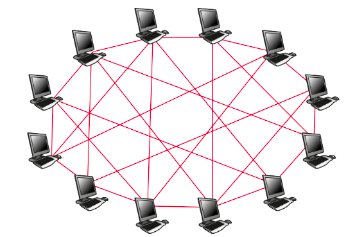
\includegraphics[scale=0.40]{modello-p2p-decentralizzato.png}}
    \hfill
    \subfloat[\emph{P2P centralizzato}]{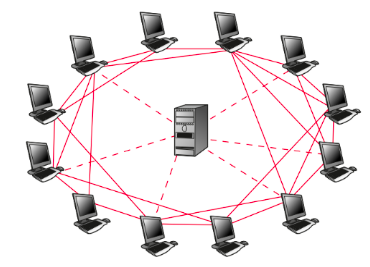
\includegraphics[scale=0.40]{modello-p2p-centralizzato.png}}
    \hfill
    \subfloat[\emph{P2P ibrido}]{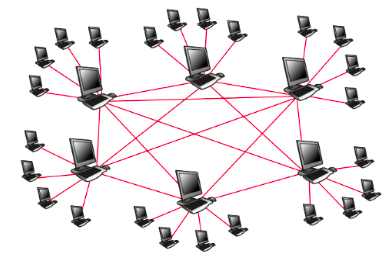
\includegraphics[scale=0.40]{modello-p2p-ibrido.png}}
    \caption{Architetture \emph{P2P} a confronto}
\end{figure}

\paragraph{Cloud computing}
Il \emph{cloud computing} è un insieme di risorse IT (hardware e software)
distribuite e accessibili attraverso la rete. In particolare, questa architettura
viene implementata come un \emph{sistema distribuito}, su diversi server dislocati
nel mondo, che vengono utilizzati per fornire un servizio.

Per accedere alle risorse i client contattano un \emph{endpoint}, cioè un server
che funge da interfaccia e che si occupa di recuperare le risorse
richieste contattando gli altri server della rete.

Questo modello porta con sé numerosi vantaggi:
\begin{itemize}
    \item \emph{Scalabilità}: è possibile aumentare o diminuire le risorse in
    base alle necessità;
    \item \emph{Velocità di configurazione}: attivare, modificare o
    disattivare un servizio è immediato;
    \item \emph{Risparmio per l'utilizzatore}: il costo varia in base all’utilizzo
    effettivo delle risorse, le quali, sono assegnate dinamicamente dal gestore
    con un sistema di \emph{provisioning dinamico} e con granularità fine;
    \item \emph{Risparmio per il fornitore}: le risorse sono virtualizzate,
    ovvero condivise tra tutti gli utilizzatori. Ciò implica che il sistema può
    avere a disposizione meno risorse di quelle che servirebbero a soddisfare le
    richieste dei client se queste venissero fatte tutte contemporaneamente (è un
    evento raro);
    \item \emph{Affidabilità}: eventuali disservizi sono risolti dal gestore e
    non dall'utilizzatore;
\end{itemize}
Ma ci sono anche delle criticità:
\begin{itemize}
    \item \emph{Sicurezza e privacy}: più utenti accedono allo stesso server per
    diverse ragioni, per cui è necessario assicurare che le attività di un utente
    non interferiscano con i dati o i processi degli altri;
    \item \emph{Problemi internazionali di natura economica e politica}: uno stato
    potrebbe decidere di impedire l'accesso ad un certo servizio offerto da un
    ente estero (e.g. servizi di Google non accessibili in Cina);
    \item \emph{Continuità del servizio offerto}: i fornitori di servizi devono
    garantire agli utenti la continua fruibilità dei propri servizi;
    \item \emph{Difficoltà di migrazione dei dati}: su un server risiedono molti
    dati per cui è complicato trasferirli da un'altra parte;
\end{itemize}
\begin{note}
    Quando si parla di \emph{scalabilità} è possibile distinguere due casi:
    \begin{itemize}
        \item \emph{Scalabilità orizzontale}: aggiungere nodi fornitori (server)
        alla rete;
        \item \emph{Scalabilità verticale}: incrementare le risorse di un singolo
        nodo;
    \end{itemize}
    Nel caso del \emph{cloud computing} viene esaltata la \emph{scalabilità
    orizzontale}.
\end{note}

\paragraph{Data center}
I fornitori di servizi cloud, dovendo gestire molti server, si appoggiano a
strutture attrezzate dove sono allocati i server di uno o più fornitori. Queste
strutture sono dette \emph{data center} e si occupano di garantire che i server
funzionino anche in caso di problemi quali, ad esempio, blackout o incendi.

\begin{figure}[ht]
    \centering
    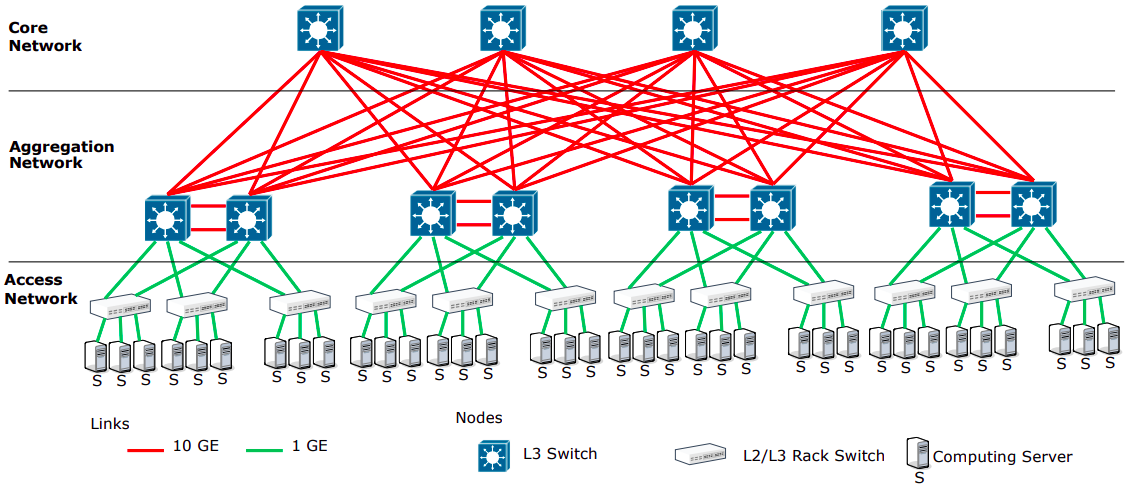
\includegraphics[width=\textwidth]{rete-data-center.png}
    \caption{Schema architetturale di un \emph{data center}}
\end{figure}
La figura sottostante mostra la struttura gerarchica della rete interna di un
\emph{data center}. In particolare, ogni server è collegato ad una rete
d'accesso; le reti d'accesso sono poi collegate ad una rete intermedia che aggrega
le comunicazioni provenienti dai server e le dirige verso la parte interna della
rete.

\paragraph{Content Delivery Network}
La struttura interna di un \emph{data center} può essere paragonata alla
struttura organizzativa dei server di grandi aziende IT come Google. Google ha 14
\emph{\quotes{mega-data center}} (\numprint{100000} server per \emph{data center})
distribuiti nel mondo che servono contenuti dinamici e personalizzati (e.g. gmail,
ricerche), 50 cluster (100-500 server per cluster) di calcolo
\emph{\quotes{bring home}} nelle reti degli \emph{IXP} che servono contenuti
statici (e.g. video di Youtube) e centinaia di cluster (decine di server per cluster)
\emph{\quotes{enter deep}} nelle reti degli \emph{ISP} che forniscono contenuti
statici (e.g. parti statiche nelle pagine dei risultati di ricerca) e permettono
il \emph{TCP splitting}.

Un'organizzazione di questo tipo permette la realizzazione di \emph{\gls{glos:CDN}},
reti \emph{\quotes{overlay}} per la diffusione di contenuti. L'idea alla base
delle \emph{CDN} è di portare i contenuti il più vicino possibile all'utente
finale in modo da ridurre la latenza, evitare colli di bottiglia e migliorare le
prestazioni generali della rete.

Esistono due tecniche per la realizzazione di \emph{CDN}:
\begin{itemize}
    \item \emph{Enter deep}: vengono installati server fisici nelle reti degli
    \emph{ISP} riducendo il ritardo e migliorando il \emph{throughput} percepito
    dagli utenti;
    \item \emph{Bring home}: vengono istallati server fisici nelle reti degli
    \emph{IXP} così da poter servire più \emph{ISP} contemporaneamente;
\end{itemize}

\section{Comunicazione in rete tra processi}
La comunicazione tra utenti si realizza come comunicazione tra processi, ovvero
programmi in esecuzione su un \emph{host}. Processi che comunicano tra loro sullo
stesso \emph{host} usano \emph{schemi interprocesso} definiti dal sistema
operativo. Quando, invece, a comunicare sono processi su \emph{host} diversi, lo
fanno mediante lo scambio di messaggi sulla rete.

Nella comunicazione in rete distinguiamo due tipi di processi:
\begin{itemize}
    \item \emph{Processi server}: forniscono un servizio e attendono di essere
    contatati da altri processi,
    \item \emph{Processi client}: usufruiscono di uno o più servizi richiedendoli
    a uno o più \emph{processi server}.
\end{itemize}

\begin{note}
    Nelle \emph{architetture P2P} le applicazioni hanno sia \emph{processi
    server} che \emph{processi client}.
\end{note}\noindent
Per realizzare la comunicazione in rete tra processi, questi devono poter essere
identificati all'interno della rete. Per farlo, è necessario conoscere gli
\emph{indirizzi IP} (indirizzi del \emph{livello Rete}) e i \emph{numeri di porta} dei
processi (indirizzi del \emph{livello Trasporto}) e questa coppia di parametri è
detta \emph{socket}.

\subsection{Socket}
\begin{definition}[Socket]
    Una socket è un'interfacci di un host, creata da un'applicazione
    e controllata dal Sistema Operativo, tramite la quale un processo di
    quell'applicazione può scambiare messaggi con il processo di un'altra
    applicazione.
\end{definition}\noindent
Le \emph{socket} sono basate sull'architettura \emph{client-server} quindi
esistono \emph{socket client} e \emph{socket server}.

La creazione e l'utilizzo delle \emph{socket} fa uso di API messe a disposizione
da una \emph{socket API} che permettono anche di scegliere
il protocollo di \emph{livello Trasporto} da utilizzare: \emph{\gls{prot:UDP}}
o \emph{\gls{prot:TCP}}.

\paragraph{Socket TCP}
Le \emph{socket TCP} utilizzando il protocollo \emph{TCP} per il trasporto
dei messaggi tra un processo e l'altro.

\begin{figure}[ht]
    \centering
    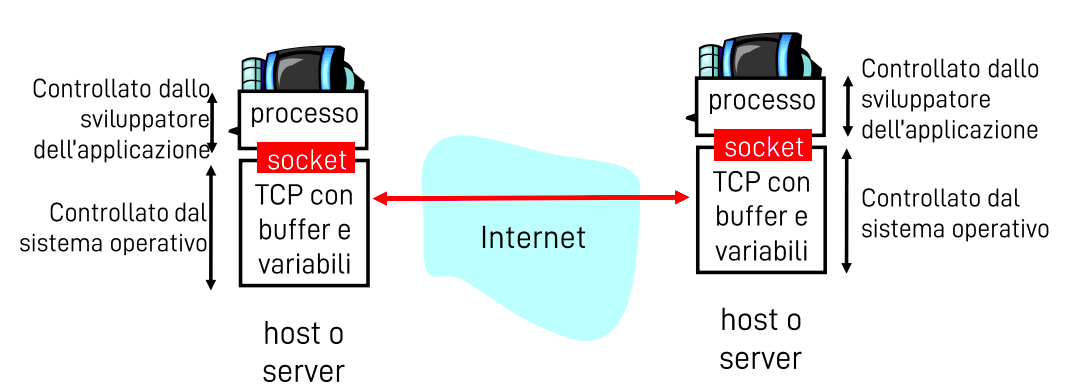
\includegraphics[width=\textwidth]{socket-tcp.png}
    \caption{Funzionamento \emph{socket TCP}}
\end{figure}\noindent
Al momento della creazione della \emph{server socket} viene specificato il
\emph{numero della porta} sulla quale il server si metterà in ascolto, mentre
nella creazione della \emph{client socket} vengono specificati
l'\emph{indirizzo IP} e il \emph{numero di porta} del processo server.

Inoltre, quando il client crea la \emph{socket} viene stabilita una connessione
\emph{TCP} con il server, il quale, risponde creando una nuova \emph{socket} per
comunicare con quel client. Questo comportamento consente al server di comunicare
con più client contemporaneamente distinguendoli in base alla
\emph{porta sorgente}\footnote{Nel corso della trattazione questo verrà reso
più chiaro}.

\begin{figure}[ht]
    \centering
    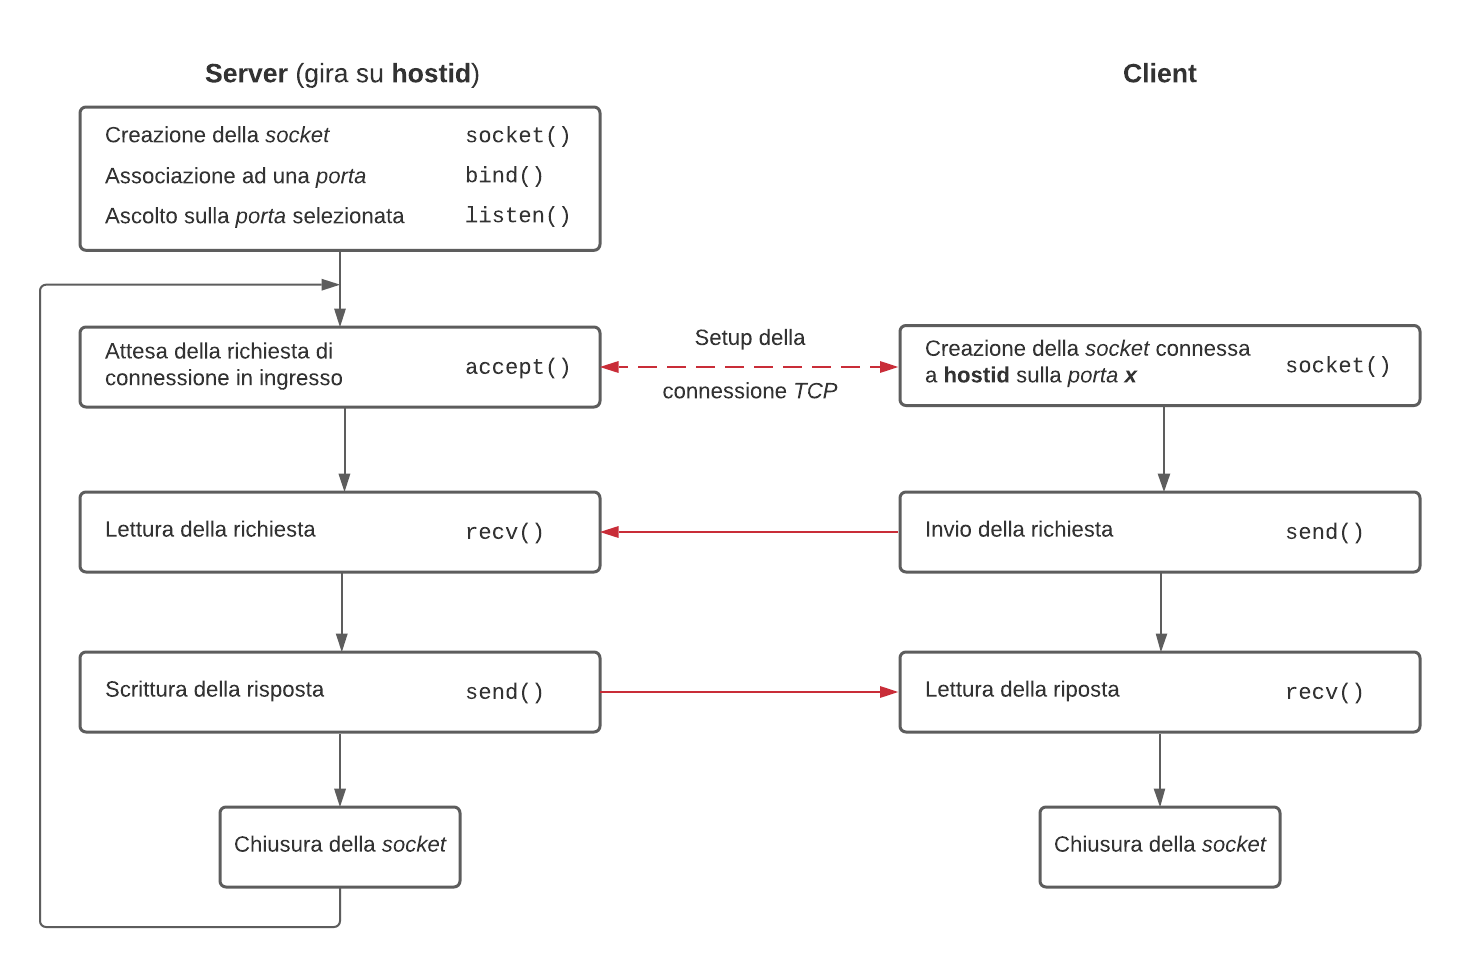
\includegraphics[scale=0.3]{socket-tcp-funzionamento.png}
    \caption{Comunicazione tra \emph{socket TCP}}
\end{figure}

\paragraph{Socket UDP}
Le \emph{socket UDP} comunicano utilizzando il protocollo \emph{UDP} e,
diversamente da quanto avviene nelle \emph{socket TCP}, il client non si connette
con il server, ma include in ogni pacchetto l'\emph{indirizzo IP} e il
\emph{numero di porta} del processo server. Di conseguenza, il server, per
distinguere i client, deve estrarre da ogni pacchetto
l'\emph{indirizzo IP} e il \emph{numero di porta} del mittente.

\section{Protocolli del livello Applicativo}
Prima di passare alla discussione sui protocolli più importanti del
\emph{livello Applicativo} è meglio chiarire la terminologia.

Una pagina web è costituita da \emph{oggetti}; un \emph{oggetto} può essere un
file \emph{\gls{glos:HTML}}, un'immagine, un file audio, \dots; una pagina web è
costituita da un file base scritto in \emph{HTML}, che solitamente include altri
oggetti referenziati; ogni oggetto è referenziato da un \emph{\gls{glos:URL}}.
\begin{definition}[URL]
    Un URL è una sequenza di caratteri che identifica univocamente una
    risorsa nella rete. La struttura di un URL è la seguente:

    \centering\scalebox{0.77}{
    {\tt
    protocollo://[username[:password]@]host[:porta][</percorso>][?querystring][\#fragment]
    }}
\end{definition}

\subsection{Protocollo HTTP}
L'\emph{\gls{prot:HTTP}} è un protocollo basato sul modello \emph{client-server}:
il ruolo di \emph{client} è ricoperto dai browser che richiedono, e ricevono,
oggetti dai \emph{server web}. La comunicazione tra \emph{client} e \emph{server}
si realizza tramite lo scambio di messaggi, che vengono scambiati sfruttando
\emph{socket TCP}. In particolare, il \emph{client} crea una connessione
\emph{TCP} sulla porta 80 del \emph{server}, il quale risponde accettando la
connessione. Questa connessione viene poi chiusa al termine dello scambio di
messaggi.

\paragraph{Connessioni persistenti e non}
Le \emph{connessioni HTTP}, ovvero le \emph{connessioni TCP} create dal
protocollo \emph{HTTP}, possono essere di due tipi:
\begin{itemize}
    \item \emph{Persistenti}: prima che la connessione venga chiusa possono
    essere trasmessi più oggetti;
    \item \emph{Non persistenti}: prima che la connessione venga chiusa viene
    trasmesso un solo oggetto;
\end{itemize}
\begin{definition}[\gls{glos:RTT}]
    È definito RTT il tempo di propagazione di andata e ritorno tra due host.
\end{definition}
\begin{note}
    Con \emph{tempo di propagazione} si intende, ad esempio, il tempo impiegato
    da un piccolo pacchetto per andare dal \emph{client} al \emph{server} e
    ritornare al \emph{client}.
\end{note}
Le \emph{connessioni non persistenti} hanno un \emph{RTT} doppio perché per ogni
oggetto va riaperta una nuova \emph{connessione TCP}. Questa caratteristica
porta anche il server a dover far fronte ad un maggiore overhead del sistema
operativo che deve gestire l'apertura di tutte quelle connessioni \emph{TCP}.
Inoltre, spesso accade che i browser aprano più connessioni in parallelo per il
trasferimento degli oggetti referenziati.

Con \emph{connessioni persistenti} tutte questi problemi non si presentano, ma
se il \emph{server} comunicasse con molti \emph{client} potrebbe terminare tutte le
porte disponibili e quindi potrebbe non poter più aprire nuove connessioni.

L'\emph{HTTP/1.0} utilizzava \emph{connessioni non persistenti}, mentre
dalla versione \emph{1.1} utilizza \emph{connessioni persistenti}.

\paragraph{Struttura dei messaggi}
Il protocollo \emph{HTTP} prevede due tipi di messaggi:
\begin{itemize}
    \item \emph{Richieste HTTP}: sono inviate dal \emph{client};
    \item \emph{Risposte HTTP}: sono inviate dal \emph{server} in risposta ad
    una richiesta;
\end{itemize}
I messaggi di \emph{richiesta} hanno la seguente struttura:
\begin{figure}[h!]
    \centering
    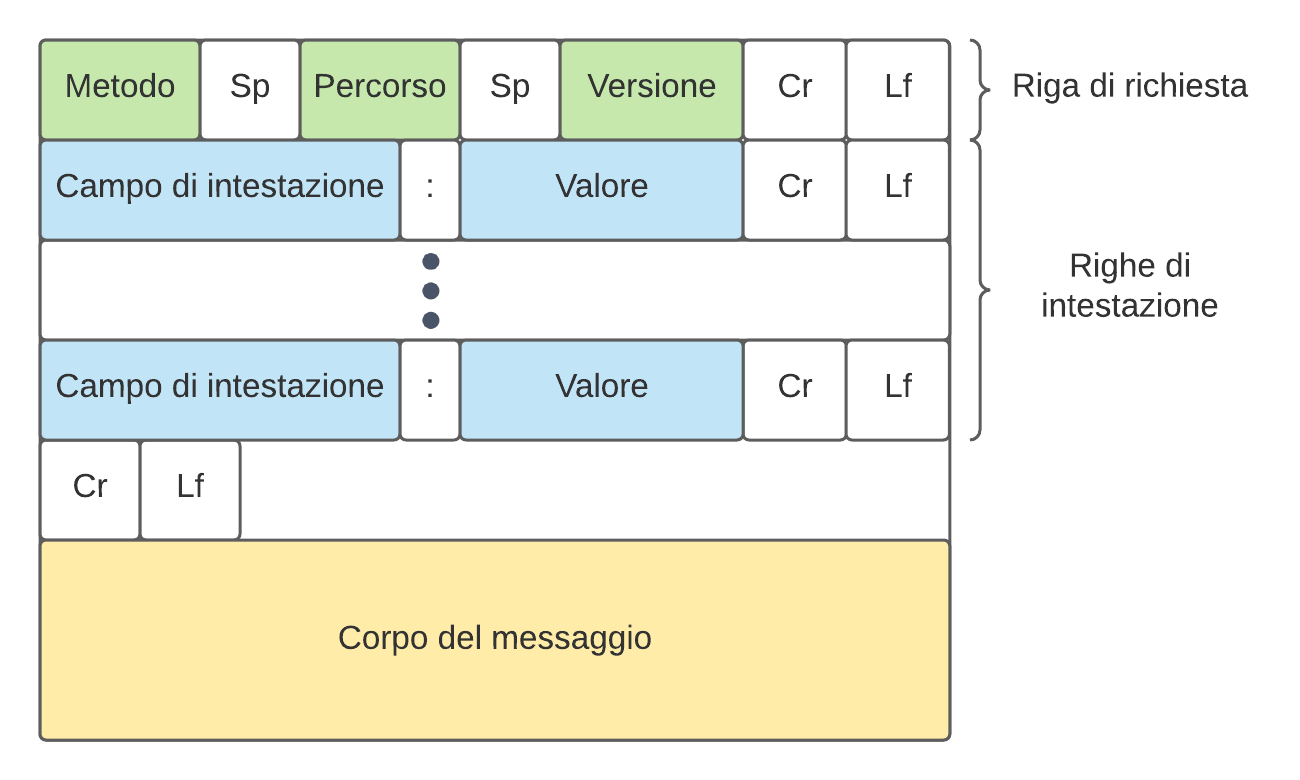
\includegraphics[width=\textwidth]{richiesta-http-struttura.png}
    \caption{Struttura messaggio di \emph{richiesta HTTP}}
\end{figure}

\noindent Il campo \emph{metodo} può essere uno dei seguenti:
\begin{itemize}
    \item \emph{GET}: richiede un file al \emph{server} scrivendo il percorso, ed
    eventuali altri dati, in chiaro nell’\emph{URL};
    \item \emph{POST}: invia informazioni all’\emph{URL} specificato scrivendo
    i dati nel corpo del \emph{messaggio HTTP};
    \item \emph{PUT}: carica un file sul \emph{server};
    \item \emph{HEAD}: richiede solo l’header della risposta senza la risorsa;
    \item \emph{OPTIONS}: richiede l’elenco dei metodi permessi dal \emph{server};
    \item \emph{DELETE}: cancella una risorsa sul \emph{server};
    \item \emph{TRACE}: traccia una richiesta visualizzando come viene trattata
    dal \emph{server};    
\end{itemize}
La \emph{versione} invece può essere uno tra: \emph{HTTP/1.0}, \emph{HTTP/1.1} e
\emph{HTTP/2.0}. Tra le \emph{righe d'intestazione} deve obbligatoriamente
essere presente il campo \emph{host} nel quale è indicato il nome dell'\emph{host}
da raggiungere.

I messaggi di \emph{risposta} hanno una struttura pressoché uguale:
\begin{figure}[ht]
    \centering
    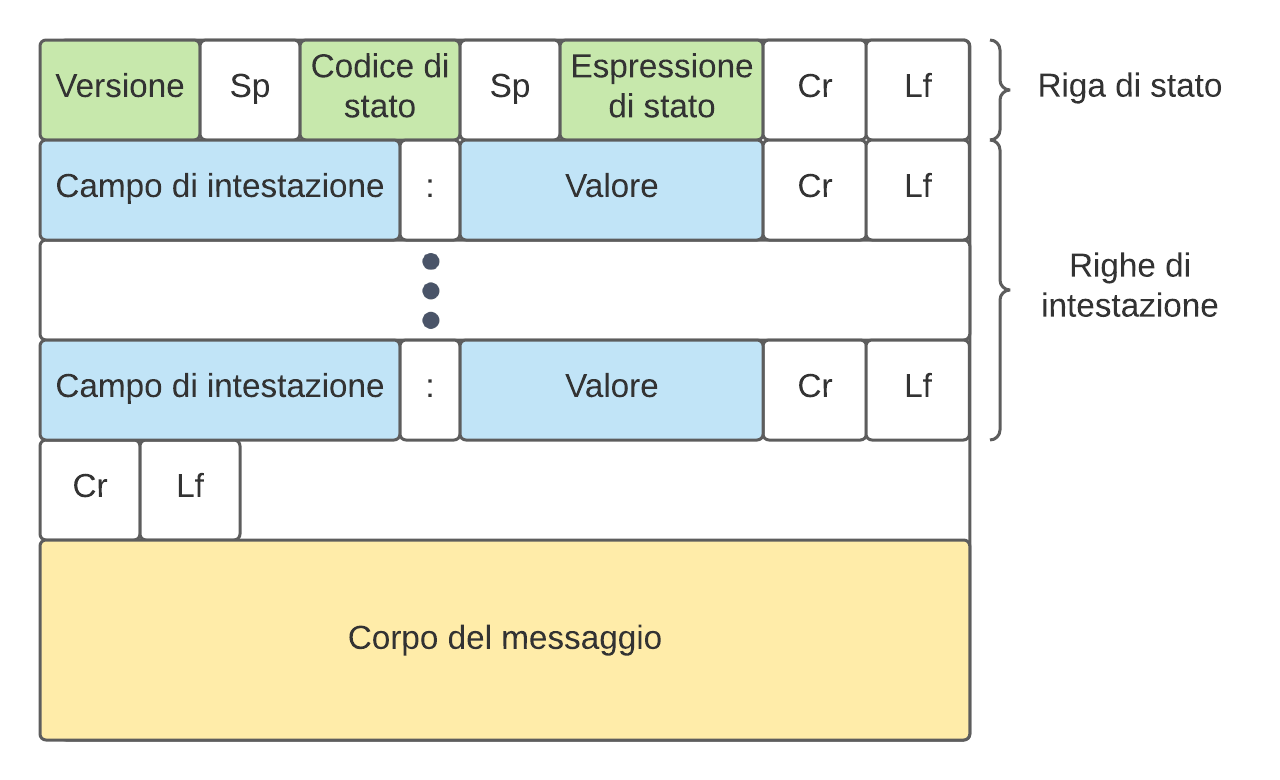
\includegraphics[width=\textwidth]{risposta-http-struttura.png}
    \caption{Struttura messaggio di \emph{risposta HTTP}}
\end{figure}

\noindent Il \emph{codice di stato} è un numero di tre cifre che identifica il
tipo di \emph{risposta} ed è definito secondo il seguente formato:
\begin{itemize}
    \item \emph{1XX}: richiesta ricevuta, risposta in arrivo;
    \item \emph{2XX}: richiesta ricevuta e soddisfatta;
    \item \emph{3XX}: ridirezione necessaria;
    \item \emph{4XX}: errore del client;
    \item \emph{5XX}: errore del server;
\end{itemize}
L'\emph{espressione di stato} è invece una descrizione del \emph{codice di stato}.

\paragraph{HTTP/2.0}
Il protocollo \emph{HTTP/2.0} è un'evoluzione dell'\emph{HTTP/1.1} ed è progettato
per ridurre la latenza percepita dall'utente e l'utilizzo delle risorse di rete
e dei server.

In particolare, l'\emph{HTTP/2.0} tenta di utilizzare un'unica connessione
tra client e server per richiedere tutte le risorse. È basato su
\emph{\gls{prot:SPDY}}, un protocollo del \emph{livello Applicativo} per il
trasporto di contenuti sul web con latenza minima. Per fare ciò, combina tre fattori:
\begin{itemize}
    \item \emph{Multiplexing di flussi}: su una singola \emph{connessione TCP}
    possono transitare un numero illimitato di flussi di dati;
    \item \emph{Priorità delle richieste}: il client può inviare un numero
    indefinito di richieste, specificando per ciascuna una priorità;
    \item \emph{Compressione dell'header HTTP}: l'header \emph{HTTP} viene
    compresso in modo da usare un minor numero di byte;
\end{itemize}
Il protocollo \emph{HTTP/2.0} introduce un livello intermedio tra il \emph{livello
Applicativo} e il \emph{Trasporto} (in realtà tra l'\emph{Applicativo} e il
\emph{Sessione}), chiamato \emph{binary framing}. Questo livello si occupa di
gestire le modalità di incapsulamento e trasferimento dei \emph{messaggi HTTP}.

\begin{figure}[h]
    \centering
    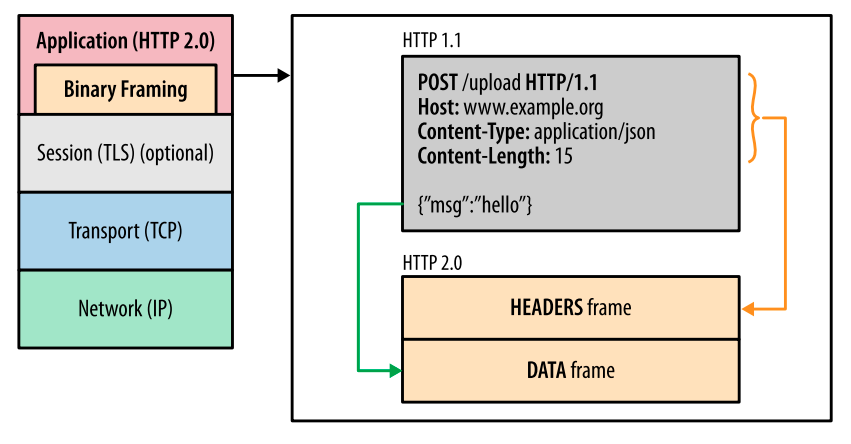
\includegraphics[width=0.7\textwidth]{binary-framing.png}
    \caption{Livello \emph{binary framing}}
\end{figure}\noindent
Il \emph{framing binario} lascia invariata la semantica dell'\emph{HTTP}, ma ne
modifica la codifica in fase di transito: ogni \emph{messaggio HTTP} è
suddiviso in \emph{frame} più piccoli codificati in binario.

\begin{note}
    Questa caratteristica dell'\emph{HTTP/2.0} lo rende incompatibile con le
    precedenti versioni, quindi server \emph{HTTP/1.x} e \emph{HTTP/2.0} non
    possono comunicare tra loro.
\end{note}\noindent
Ogni \emph{frame} è identificato da un valore univoco ed eventualmente anche da
un livello di priorità. Ogni messaggio trasmesso, che sia una richiesta o una
risposta, può essere suddiviso in uno o più \emph{frame} e ogni \emph{frame}
trasporta un tipo specifico di dati: \emph{header} o \emph{payload}.

\newpage
\begin{figure}[h]
    \centering
    \subfloat{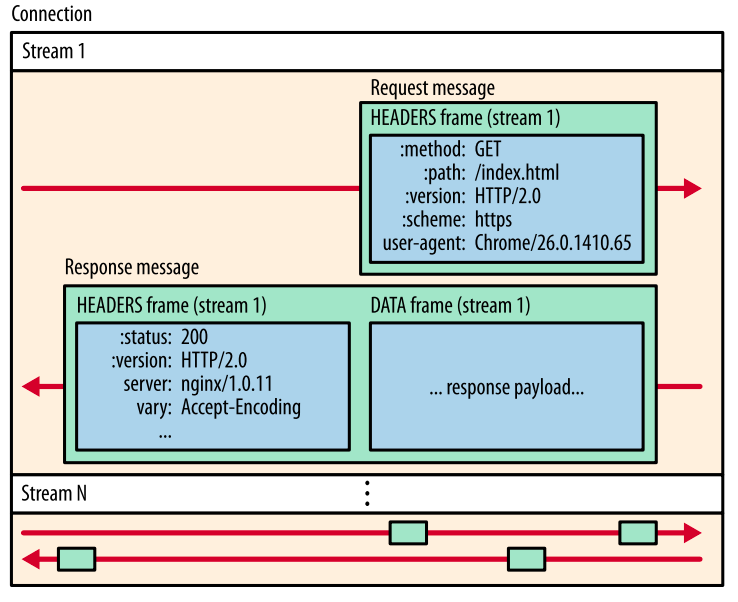
\includegraphics[scale=0.3, valign=c]{http2-stream.png}}
    \hfill
    \subfloat{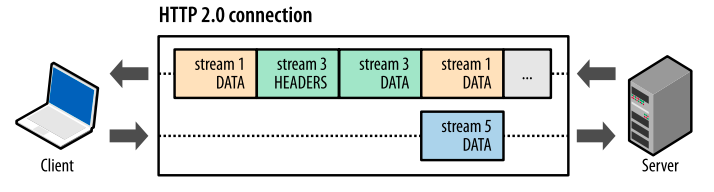
\includegraphics[scale=0.35, valign=c]{http2-frame.png}}
    \caption{Trasmissione dei \emph{frame} negli \emph{stream}}
\end{figure}

\bigskip\hspace{-0.5cm} Tutte le comunicazioni avvengono all'interno di un'unica
\emph{connessione TCP} che può trasportare un numero illimitato di \emph{stream}
bidirezionali di byte. Su ogni \emph{frame} è indicato l'identificativo unico
dello \emph{stream} sul quale sta viaggiando e questo consente di inviare i
\emph{frame} in modo indipendente, intervallandoli e ricomponendoli all'arrivo.

L'ordine di invio dei \emph{frame} dipende, qualora sia stata impostata, dalla
priorità indicata in senso crescente con un numero da 1 a 256. L'ordine di invio
dei \emph{frame} viene deciso dal server in base alle indicazioni fornitegli dal
client tramite un \emph{albero di priorità}.

\bigskip In \emph{HTTP/2.0} esiste quindi una sola \emph{connessione TCP
persistente}.

\begin{figure}[h!]
    \centering
    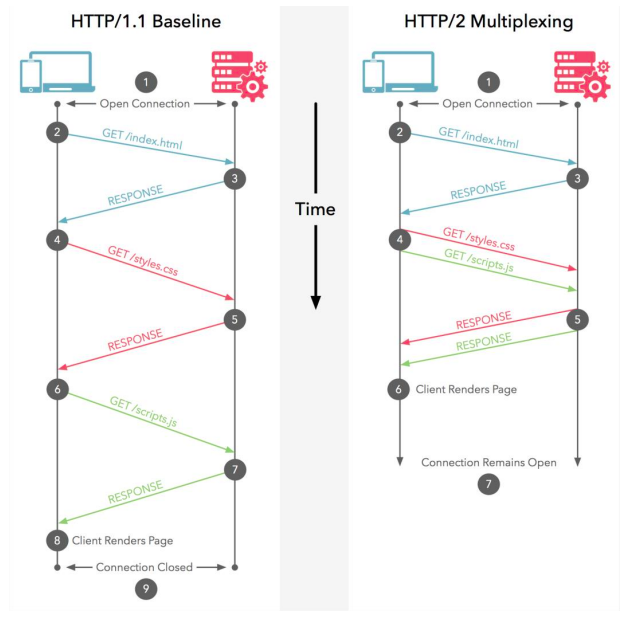
\includegraphics[width=0.7\textwidth]{http2-connessione.png}
    \caption{Connessione \emph{HTTP/1.1} VS \emph{HTTP/2}}
\end{figure}\noindent
Per tentare di ridurre ulteriormente la latenza, l'\emph{HTTP/2.0} introduce il
concetto di \emph{server push}. Quando il client fa una richiesta al server, questo
oltre alla risorsa richiesta invia anche altre risorse ad essa collegate. Queste
risorse inviate in più dal server sono dette \emph{server promise}.

\begin{figure}[h]
    \centering
    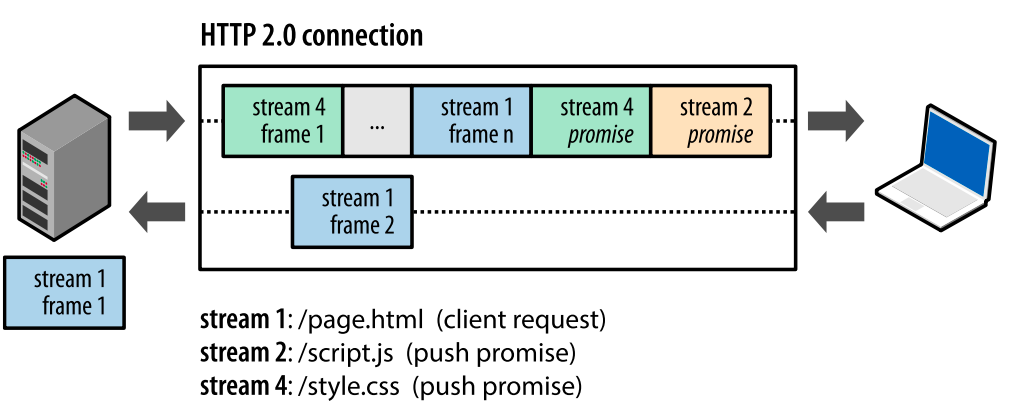
\includegraphics[width=0.7\textwidth]{http2-server-push.png}
    \caption{\emph{HTTP/2.0 server push}}
\end{figure}

\paragraph{Comunicazioni senza stato e i cookie}
Nell'\emph{HTTP} la comunicazione tra client e server è priva di stato, ciò
significa che il server non ha memoria delle precedenti richieste di un client.

Per simulare lo stato si usano i \emph{cookie}, ovvero file generati dal web
server e salvati sul client che contengono, tra le altre cose, informazioni sulle
preferenze di un client riguardo un sito web (e.g. carrello della
spesa nei siti di e-commerce).

In particolare, i \emph{cookie} sono file contenenti una stringa di testo, una
data di scadenza e un pattern per il riconoscimento dei domini di destinazione
che vengono inviati al web server ogni volta che il client accede ad una pagina
del sito.
La stringa di testo contenuta in un cookie è detta \emph{chiave di sessione} ed
è utilizzata per identificare in modo univoco un client e i relativi dati
che vengono salvati in un database accessibile al server web.

\begin{figure}[h]
    \centering
    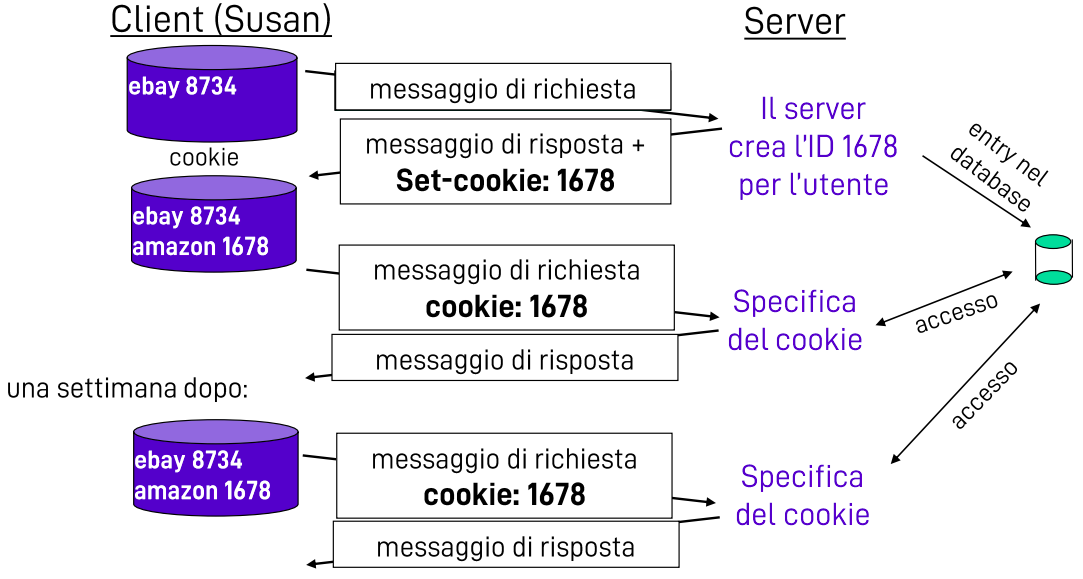
\includegraphics[width=\textwidth]{http-cookie.png}
    \caption{Utilizzo dei \emph{cookie}}
\end{figure}\noindent
La prima volta che un client accede ad una pagina web, il server crea una
\emph{chiave di sessione} e ne specifica il valore nel campo \emph{Set-cookie}
dell'\emph{header HTTP} del messaggio di risposta. Il browser del client salva
quel valore e nelle successive richieste lo va ad inserire nell'\emph{header}
nel campo \emph{Cookie}.

\paragraph{Server proxy}
Il \emph{proxy} è un server intermedio che si pone tra client e server.
Quando un client richiede una risorsa al server, la richiesta viene prima
intercettata dal \emph{proxy} che verifica la presenza della risorsa nella propria
cache interna. Se nel \emph{proxy} la risorsa richiesta non è presente o non è
aggiornata, la richiesta viene inoltrata dal \emph{proxy} al server di destinazione.

Quindi, il \emph{proxy} riceve la risposta dal server e prima di inviarla al
client, provvede a salvarla al suo interno, così da poterla riutilizzare per future
richiese senza dover ricontattare il server.

Tuttavia, nel caso di risorse dinamiche è importante che queste siano aggiornate,
quindi quando il \emph{proxy} riceve una richiesta, invia un \emph{messaggio HTTP}
di tipo \emph{HEAD} al web server e confronta la data di ultima modifica della
pagina salvata con quella della pagina sul web server. Se la pagina salvata è
scaduta, il \emph{proxy} la aggiorna e risponde alla richiesta del client
con la versione aggiornata. In alternativa ad una richiesta \emph{HEAD} seguita
da una \emph{GET}, il \emph{proxy} può utilizzare una \emph{GET condizionale} che
richiede la risorsa solo se la data di ultima modifica è successiva a quella
indicata nell'\emph{header} nel campo \emph{If-modified-since}.

\begin{figure}[h]
    \centering
    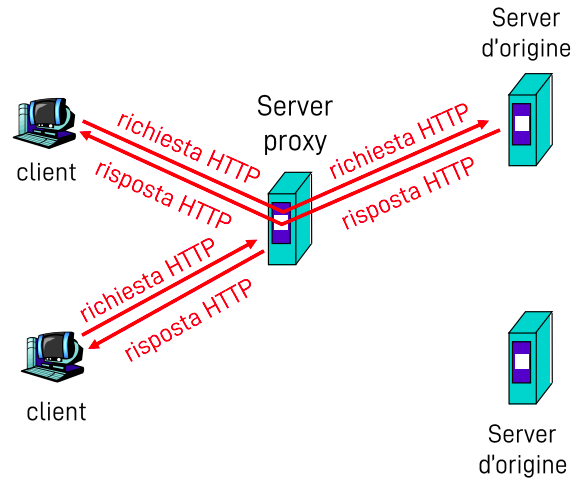
\includegraphics[width=0.7\textwidth]{http-proxy.png}
    \caption{Server \emph{proxy}}
\end{figure}

\subsection{Protocollo FTP}
L'\emph{\gls{prot:FTP}} è un protocollo \emph{client-server} per il trasferimento
di file tra client e server. Vengono usate due connessioni \emph{TCP} sulle
porte 21 e 22 del server. La prima è dedicata allo scambio dei comandi, mentre la
secondo, viene aperta all'occorrenza e viene mantenuta attiva soltanto per il
tempo necessario, ed è usata per il trasferimento dei file.

\begin{figure}[ht]
    \centering
    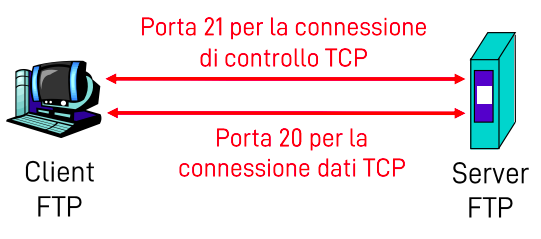
\includegraphics[width=0.7\textwidth]{ftp.png}
    \caption{Connessioni aperte dall'\emph{FTP}}
\end{figure}

\newpage
\subsection{Protocolli per la posta elettronica}
Nello scambio di messaggi di posta elettronica gli attori principali sono tre:
\begin{itemize}
    \item \emph{Agente utente}: permette la composizione e la lettura delle email;
    \item \emph{Server di posta}: contiene i messaggi da recapitare all'utente e la
    coda di messaggi da trasmettere;
    \item \emph{Protocollo di trasferimento}: gestisce il trasporto di email tra
    utente e server e tra server;
\end{itemize}

\paragraph{Protocollo SMTP}
È utilizzato per mettere in comunicazione i \emph{server di posta} e, in particolare,
trasmette i messaggi direttamente tra il server mittente e il server destinatario.
Il trasferimento è articolato in tre fasi: \emph{handshake}, \emph{trasferimento}
e \emph{chiusura}.

L'interazione tra i server avviene mediante messaggi in formato ASCII a 7 bit; ad
ogni comando corrisponde un messaggio di risposta formato da un codice di stato e
un'espressione. Inoltre, l'\emph{\gls{prot:SMTP}} trasmette più oggetti all'interno
di uno stesso messaggio e utilizza \emph{connessioni persistenti}.

\begin{figure}[h!]
    \centering
    \begin{lstlisting}[basicstyle=\scriptsize]
        S: 220 hamburger.edu
        C: HELO crepes.fr
        S: 250 Hello crepes.fr, pleased to meet you
        C: MAIL FROM: <alice@crepes.fr>
        S: 250 alice@crepes.fr... Sender ok
        C: RCPT TO: <rob@hamburger.edu>
        S: 250 rob@hamburger.edu ... Recipient ok
        C: DATA
        S: 354 Enter mail, end with "." on a line by itself
        C: From: alice@crepes.fr
        C: To: bob@hamburger.edu
        C: Subject: Important question.
        C: 
        C: Do you like ketchup?
        C: .
        S: 250 Message accepted for delivery
        C: QUIT
        S: 221 hamburger.edu closing connection
    \end{lstlisting}
    \caption{Esempio di interazione tra \emph{server SMTP}}
\end{figure}\noindent
È possibile trasmettere anche oggetti multimediali utilizzando l'estensione
\emph{MIME} e codificando i dati da trasmettere usando la codifica \emph{base64}
che rappresenta 6 bit usandone 8.

Per utilizzare l'estensione \emph{MIME} è sufficiente aggiungere nell'intestazione
del messaggio le seguenti tre righe:
\newpage
\begin{figure}[ht]
    \centering
    \begin{lstlisting}[basicstyle=\scriptsize]
        MIME-Version: 1.0
        Content-Transfer-Encoding: base64
        Content-Type: image/jpeg
    \end{lstlisting}
    \caption{Intestazione per messaggi multimediali}
\end{figure}\noindent
Ovviamente il \texttt{Content-type} dipende dal tipo di oggetto che si vuole
trasferire.

\paragraph{Protocolli POP3 e IMAP4}
\emph{\gls{prot:POP}} e \emph{\gls{prot:IMAP}} sono usati per il trasferimento
di messaggi tra \emph{server} e \emph{agenti utente}. Entrambi utilizzano
il protocollo \emph{\gls{prot:TCP}} per lo scambio di messaggi, ma a parte questo
sono basati su filosofie opposte.

Il protocollo \emph{POP3} prevede che l'utente si colleghi al server e scarichi
tutte le email disponibili. Una volta scaricate, le email vengono eliminate dal
server. D'altra parte, il protocollo \emph{IMAP4} consente all'utente di accedere
alle email mantenendole nel server e inoltre permette l'organizzazione dei
messaggi in cartelle. Per questo motivo, l'\emph{IMAP4} mantiene lo stato
dell'utente tra le varie sessioni, mentre il \emph{POP3} no.

\begin{figure}[h!]
    \centering
    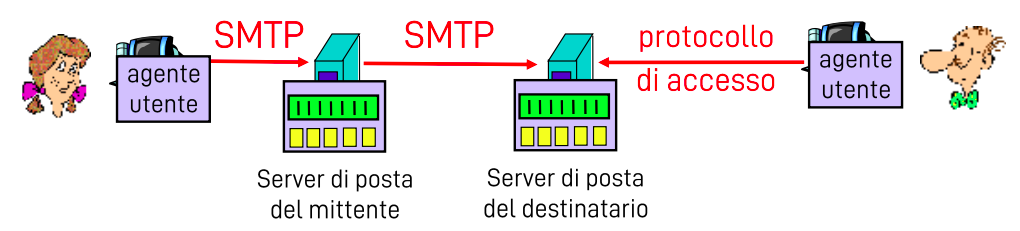
\includegraphics[width=\textwidth]{email.png}
    \caption{Scambio di email}
\end{figure}

\begin{note}
    Ci si potrebbe chiedere perché non si usi soltanto l'\emph{SMTP}.
    La risposta è che l'\emph{SMTP} può trasmettere un messaggio soltanto se
    il ricevente è online.
\end{note}

\paragraph{Protocollo TLS}
Il \emph{\gls{prot:TLS}} è un protocollo che consente di rendere sicura la
comunicazione tra due entità fornendo:
\begin{itemize}
    \item \emph{Autenticazione}: l'identità di mittente e destinatario viene
    verificata;
    \item \emph{Integrità dei dati}: viene garantito che il messaggio non verrà
    manipolato durante la trasmissione;
    \item \emph{Confidenzialità}: soltanto il legittimo destinatario sarà in
    grado di accedere al contenuto del messaggio;
\end{itemize}
Il funzionamento del \emph{TLS} può essere suddiviso in tre fasi:
\emph{negoziazione fra le parti dell'algoritmo da utilizzare}, \emph{scambio delle
chiavi e autenticazione}, \emph{cifratura simmetrica e autenticazione dei messaggi}.

È possibile combinare i tre protocolli per lo scambio di email con il
\emph{TLS} per rendere sicuro lo scambio di messaggi. Ovviamente, un \emph{host}
che non utilizza questa tecnologia non può comunicare con un altro \emph{host} che
la usa, quindi, vengono usati \emph{numeri di porta} diversi dalle versioni
\quotes{non sicure} di quei protocolli.

\bigskip\noindent
Esiste un'evoluzione del \emph{TLS} chiamata \emph{STARTTLS} che consente
di comunicare sulle porte originali dei protocolli. In particolare, il client
che intende assicurare la comunicazione, chiede al server l'instaurazione di una
connessione cifrata, la sessione inizia in chiaro e diventa cifrata prima che
vengano trasmessi dati sensibili.

\subsection{Protocollo DNS}
Ad ogni \emph{nome di dominio} è associato un \emph{indirizzo IP} (in realtà anche
più di uno); il protocollo \emph{\gls{prot:DNS}} consente di risolvere i \emph{nomi
di dominio}, ovvero di risalire all'\emph{indirizzo IP} associato a un \emph{nome}.
Oltre a ciò, altri servizi offerti dal \emph{DNS} sono:
\begin{itemize}
    \item \emph{Host aliasing}: è possibile associare degli alias ad un \emph{nome
    di dominio};
    \item \emph{Mail server aliasing}: come per l'\emph{host aliasing}, ma per i
    server mail;
    \item \emph{Load distribution}: il \emph{DNS} può essere usato per distribuire
    il carico delle richieste tra più server replicati, cioè con lo stesso nome.
    Ciò è possibile perché quando un \emph{server DNS} riceve una richiesta,
    restituisce, se possibile, più di un \emph{indirizzo IP}. L’ordine degli
    \emph{indirizzi IP} dei server replicati viene cambiato ad ogni richiesta in
    modo da evitare che le richieste arrivino sempre ad unico server, congestionandolo;
\end{itemize}

\paragraph{Struttura dei nomi di dominio}
Prima di procedere oltre è bene chiarire i termini usati per descrivere i
\emph{nomi di dominio}. Il nome \texttt{drive.google.com.}, ad esempio, si
struttura, a partire da destra, in:
\begin{itemize}
    \item \emph{Root}: è implicito in ogni nome ed è indicato con un punto
    \texttt{(.)};
    \item \emph{\gls{glos:TLD}}: è il \emph{dominio di primo livello} e può
    essere generico (e.g. \texttt{.com}, \texttt{.org}, \dots) o nazionale (e.g.
    \texttt{.it}, \texttt{.de}, \dots);
    \item \emph{\gls{glos:SLD}}: è il \emph{dominio di secondo livello}
    (\texttt{.google});
    \item \emph{Sottodominio}: è un sottodominio del \emph{SLD} e server ad
    indentificare uno specifico \emph{host} o gruppo di \emph{host} all'interno
    del dominio (\texttt{drive});
\end{itemize}

\paragraph{Implementazione del DNS}
Il \emph{DNS} è implementato come una gerarchia di database distribuiti.
Partendo dal vertice, la gerarchia di server DNS è organizzata in tre livelli:
\begin{itemize}
    \item \emph{Root server}: sono 13 in tutto il mondo e conoscono la posizione
    dei server che gestiscono i \emph{TLD};
    \item \emph{TLD server}: gestiscono i \emph{TLD} e conoscono la posizione degli
    \emph{authoritative server} (\emph{server di competenza}) che gestiscono i
    \emph{SLD} di una determinata zona;
    \item \emph{Authoritative server}: gestiscono i \emph{SLD} e sanno risolvere
    tutti i nomi di dominio della loro zona di competenza;
\end{itemize}
Esistono 13 \emph{root server} logici nel mondo, ma ognuno di essi è pesantemente
ridondato per evitare interruzioni di servizio o perdite di dati. Anche i
\emph{TLD} e gli \emph{authoritative server} sono ridondati per scongiurare
congestioni, sovraccarichi e gli altri problemi visti per i \emph{root server}.

Oltre ai server della gerarchia, ogni \emph{\gls{glos:ISP}} ha un proprio
\emph{server DNS locale} detto \emph{default name server} che riceve le richieste
fatte dagli \emph{host} della rete, le inoltra ai server della gerarchia e infine
restituisce all'\emph{host} interessato il risultato dell'interrogazione.

Gli \emph{host} interrogano i \emph{server DNS} sfruttando le funzioni fornite da
un \emph{resolver}. Si tratta di un’applicazione client, generalmente integrata
nel sistema operativo, che permette di realizzare la risoluzione dei \emph{nomi di
dominio}.

\begin{note}
    Ci si potrebbe chiedere perché non venga usato un unico server centralizzato.
    Il motivo è che una soluzione del genere comporterebbe enormi problematiche,
    quali:
    \begin{itemize}
        \item \emph{\gls{glos:SPOF}}: il server diventerebbe un \emph{SPOF} col
        risultato che un suo guasto renderebbe il servizio inutilizzabile in
        tutta la rete;
        \item \emph{Volume di traffico}: dovendo gestire le richieste di tutta la
        rete il server sarebbe costantemente congestionato;
        \item \emph{Distanza}: il server sarebbe stato distante dalla maggior parte
        degli utenti e per alcuni addirittura irraggiungibile per via del limite di
        \emph{hop};
        \item \emph{Manutenzione permanente}: il server dovrebbe essere costantemente
        aggiornato per aggiungere e modificare i dati esistenti rendendolo
        inutilizzabile per la maggior parte del tempo;
        \item \emph{Non scalabilità}: il server avrebbe avuto molte difficoltà ad
        adattarsi ai mutamenti del volume di traffico della rete;
    \end{itemize}
\end{note}

\begin{figure}[h]
    \centering
    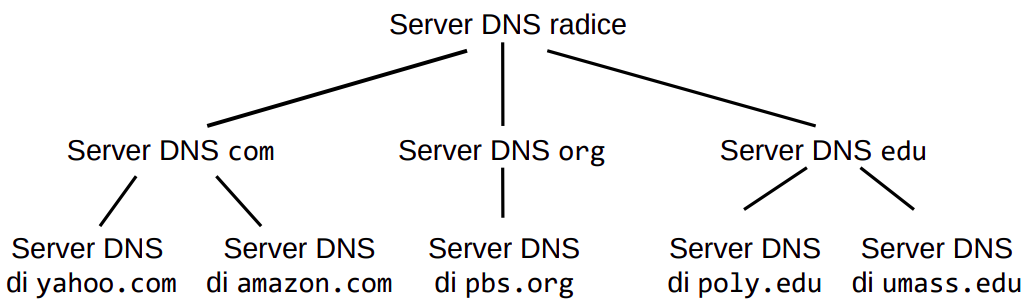
\includegraphics[width=\textwidth]{gerarchia-dns.png}
    \caption{Gerarchia dei \emph{server DNS}}
\end{figure}

\paragraph{Interrogare i server}
Quando un \emph{host} intende risolvere un \emph{nome di dominio} contatta il
proprio \emph{default name server}. Se questo ha già la risposta all'interrogazione
ricevuta, la restituisce direttamente all'\emph{host}, altrimenti interroga la
gerarchia. Per fare questo esistono due modalità: \emph{iterativa} e \emph{ricorsiva}.

Nella modalità \emph{iterativa} il \emph{server DNS locale} procede ad interrogare
ogni livello della gerarchia. Partendo dal \emph{root server}, richiede l'indirizzo
del \emph{TLD server} associato al \emph{TLD} da risolvere, quindi interroga il
\emph{server di competenza} per il \emph{nome} completo.

D'altra parte, nella modalità \emph{ricorsiva}, il \emph{server DNS locale}
interroga il \emph{root server}, questo quindi interroga il \emph{TLD server} che
a sua volta interroga l'\emph{authoritative server}. Una volta trovata la risposta
questa risale la gerarchia fino a tornare al \emph{default name server}.

Solitamente i \emph{server DNS} non rispondono a richieste fatte in modalità
\emph{ricorsiva} perché sono causa di congestione.

\newpage
\begin{figure}[ht]
    \centering
    \subfloat[Query \emph{iterativa}]{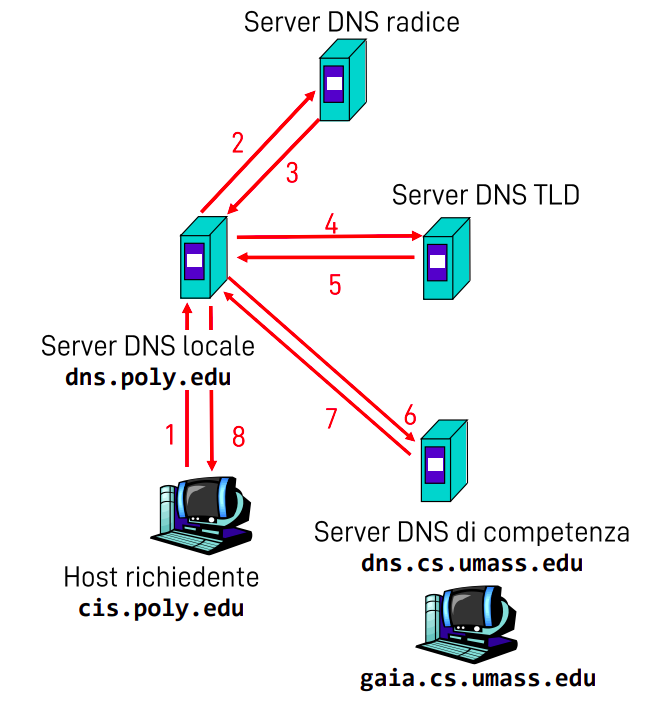
\includegraphics[width=0.5\textwidth]{query-iterativa.png}}
    \hfill
    \subfloat[Query \emph{ricorsiva}]{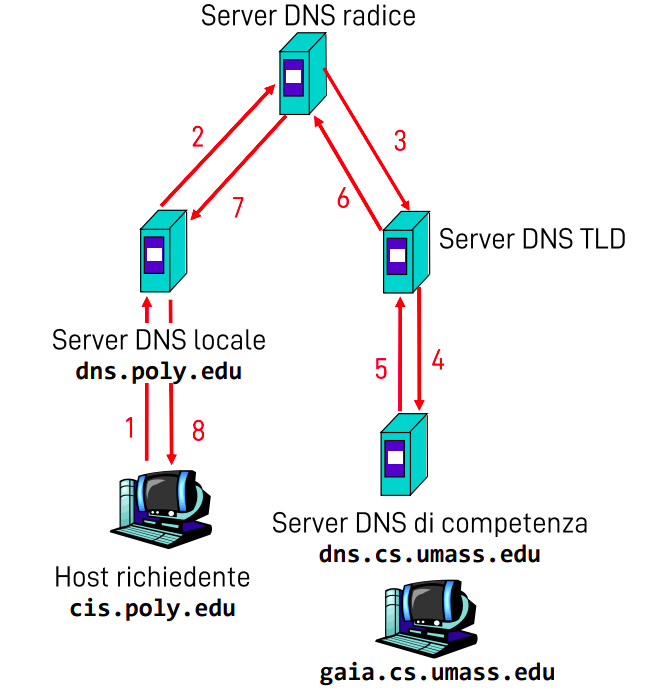
\includegraphics[width=0.5\textwidth]{query-ricorsiva.png}}
    \caption{Query \emph{iterativa} VS query \emph{ricorsiva}}
\end{figure}

\paragraph{DNS caching}
Quando un \emph{server DNS} impara la mappatura di una di un \emph{nome di dominio},
la salva in una cache. Queste informazioni vengono invalidate dopo un certo periodo
di tempo in modo da costringere l'aggiornamento dei dati.

Solitamente, per evitare di contattare i \emph{root server}, i \emph{server DNS
locali} salvano gli indirizzi dei \emph{TLD server}.

\paragraph{Resource record}
I \emph{server DNS} memorizzano le informazioni in \emph{\gls{glos:RR}} con questo
formato:
\[\texttt{(name, value, type, ttl)}\]
I valori più comuni per il campo \texttt{type} sono:
\begin{itemize}
    \item \texttt{A}: associa il \emph{nome di dominio} a un indirizzo \emph{IPv4}
    (\texttt{name}: \emph{nome di dominio}, \texttt{value}: \emph{indirizzo IPv4});
    \item \texttt{AAAA}: come il precedente, ma associa un indirizzo \emph{IPv6};
    \item \texttt{CNAME}: associa un \emph{alias} al \emph{nome canonico}
    (\texttt{name}: \emph{alias}, \texttt{value}: \emph{nome canonico});
    \item \texttt{MX}: associa a un \emph{nome di dominio} il proprio \emph{mail
    server} (\texttt{name}: \emph{nome di dominio}, \texttt{value}: nome del
    \emph{mail server});
    \item \texttt{NS}: associa al \emph{nome di dominio} il nome del relativo
    \emph{server di competenza} (\texttt{name}: \emph{dominio}, \texttt{value}:
    nome del \emph{server di competenza});
\end{itemize}

\paragraph{Messaggi DNS}
Il protocollo \emph{DNS} prevede due tipi di messaggi: \emph{domande} e
\emph{risposte}. Entrambi usano lo stesso formato.

\newpage
\begin{figure}[ht]
    \centering
    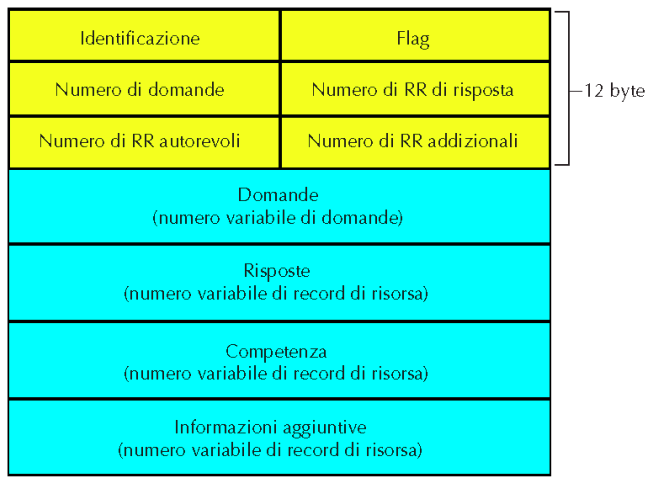
\includegraphics[width=0.7\textwidth]{messaggio-dns.png}
    \caption{Struttura di un messaggio \emph{DNS}}
\end{figure}\noindent
I campi descrivono:
\begin{itemize}
    \item \emph{Identificazione}: un valore di 16 bit che identifica in modo
    univoco una domanda e la relativa risposta;
    \item \emph{Flag}: i flag sono quattro:
    \begin{itemize}
        \item \emph{Domanda o risposta};
        \item \emph{Richiesta di ricorsione};
        \item \emph{Ricorsione disponibile};
        \item \emph{Risposta di competenza};
    \end{itemize}
    \item \emph{Domande}: campi per il \emph{nome} richiesto e il tipo di domanda;
    \item \emph{Risposte}: \emph{RR} di risposta alla domanda;
    \item \emph{Competenza}: \emph{RR} dedicati per i \emph{server di competenza};
    \item \emph{Informazioni aggiuntive}: informazioni extra che possono essere
    usate;
\end{itemize}

\paragraph{Inserire record nel database}
Quando si registra un \emph{nome di dominio} presso un \emph{registrar}, ovvero
una società che garantisce l'unicità del \emph{nome}, questa provvede ad inserire
nel database del \emph{server DNS} due \emph{RR}. Nel primo viene associato il
\emph{nome di dominio} al relativo \emph{server di competenza}, mentre nel
secondo associa il nome del \emph{server di competenza} al suo \emph{indirizzo IP}.